\documentclass[6pt]{../../shared/AiTex}
\usepackage{csvsimple}

\title{Memoria entrega 4}
\author{A.L.K.}
\date{Febrero 2024}

\begin{document}
%\datos{facultad}{universidad}{grado}{asignatura}{subtitulo}{autor}{curso}
\datos{Informática}{Universidad Complutense de Madrid}{Ingeniería informática}{Aprendizaje Automatico y Big Data}{Entrega 4: clasificación multi-clase}{Alejandro Barrachina Argudo}{2023-2024}
% \portadaApuntes
% \pagestyle{empty}
% \tableofcontents
% \pagestyle{empty}
\justify

\begin{center}

    {\huge \textbf{\underline{\subtitulo}}} \\
    { \lesson - \autor}

\end{center}


\section*{Introducción}

En este documento se explicará el código del entregable 4 y el proceso del clasificador multi-clase. Esta práctica se divide en 2 apartados: clasificador multi-clase y redes neuronales. El \textit{dataset} consiste de imágenes de números escritos a mano como los vistos en la figura \ref{fig:digitos}

Para esta práctica se usarán los siguientes \textit{imports} vistos en la figura \ref{fig:imports}. Parte del código se reutiliza de la práctica anterior. A los \textit{strings} estáticos anteriores añadimos uno para guardar el modelo entrenado (figura \ref{fig:strings})
\begin{figure}[H]
    \centering
    \lstinputlisting[firstline=1,lastline=7, style=custompython]{../multi_class.py}
    \caption{Código de las bibliotecas usadas}
    \label{fig:imports}
\end{figure}

\begin{figure}[H]
    \centering
    \lstinputlisting[firstline=9,lastline=9, style=custompython]{../multi_class.py}
    \caption{Código de los nuevos strings estáticos}
    \label{fig:strings}
\end{figure}

\begin{figure}[H]
    \centering
    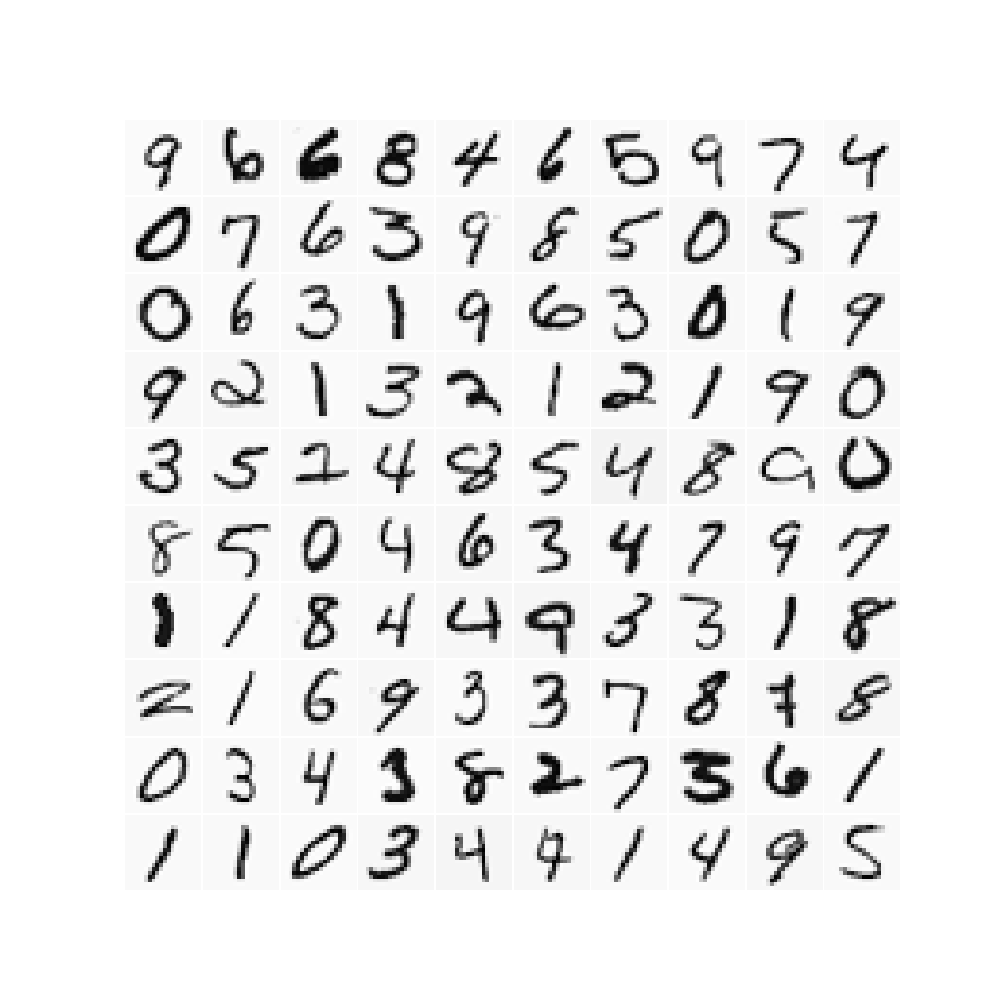
\includegraphics[width=0.5\textwidth]{./imagenes/data.png}
    \caption{Ejemplo de los dígitos del \textit{dataset}}
    \label{fig:digitos}
\end{figure}

\section{Parte A: clasificación multi-clase}

Para esta sección vamos a reutiliza todo lo referente a la regresión logística de la práctica anterior. Los cambios implementados son la distinción entre clases distintas y la concurrencia para acortar los tiempos de entrenamiento.

Para la concurrencia usaremos 3 funciones distintas: \textit{train\_model}, \textit{train\_all} y \textit{oneVsAll} (figuras \ref{fig:train_model}, \ref{fig:train_all} y \ref{fig:oneVsAll} respectivamente). La función \textit{train\_model} es la misma que la de la práctica anterior, pero ahora se le pasa un parámetro extra, \textit{class\_num}, que indica la clase que se está entrenando. La función \textit{train\_all} se encarga de generar los hilos para entrenar cada etiqueta y juntar todos los resultados. La función \textit{train\_model} se encarga de generar los datos de entrenamiento ($\alpha$, $\lambda$ y el número de iteraciones.) La función \textit{oneVsAll} hace de wrapper para las dos funciones anteriores. Finalmente, la función \textit{run\_one\_vs\_all} (figure \ref{fig:run_one_vs_all}) se encarga de hacer de driver para esta sección.

Tras esto, utilizamos la función \textit{predictOneVsAll} (figura \ref{fig:predictOneVsAll}) para predecir la clase de un conjunto de datos. Esta función es muy similar a la de la práctica anterior, pero ahora diferencia entre los distintos tipos de clases dadas según el \textit{dataset}. La función \textit{run\_one\_vs\_all} será la función principal de este apartado. Cargaremos los datos del \textit{dataset} desde aquí y daremos valores al número de clases y a $\lambda$, así como mostraremos los distintos gráficos y predicciones.

Para la elaboración de los gráficos usaremos las funciones \textit{plot\_confusion\_matrix} (figura \ref{fig:plot_confusion_matrix}) para hacer la matriz de confusión (figura \ref{fig:matrix_a}) y \textit{print\_predictions} (figura \ref{fig:print_predictions}) para mostrar las predicciones a lo largo del entrenamiento (figura \ref{fig:predictions_a}).

Tras una sesión de entrenamiento con $\alpha = 0.2$, $\lambda = 0.01$ y 2500 iteraciones, obtenemos una predicción del 94.7\%, con estos gráficos (matriz de confusión \ref{fig:matrix_a} y predicciones \ref{fig:predictions_a}) para ver mejor los resultados. Con la función \textit{save\_model} (figura \ref{fig:save_model}) guardamos el modelo para futuras predicciones y para evitar nuevos entrenamientos. Las funciones \textit{save\_predict} y \textit{save\_last\_predictions} (figura \ref{fig:save_predict} y \ref{fig:save_last_prediction}) guardan las predicciones en distintos tipos de archivo para poder usarlos en otras ocasiones para hacer gráficos.

Las últimas predicciones de cada label son:

% leemos el csv de datos y lo trasponemos para hacer una tabla vertical
\csvautotabular{../models/one_vs_all_predict.csv}

\begin{figure}[H]
    \centering
    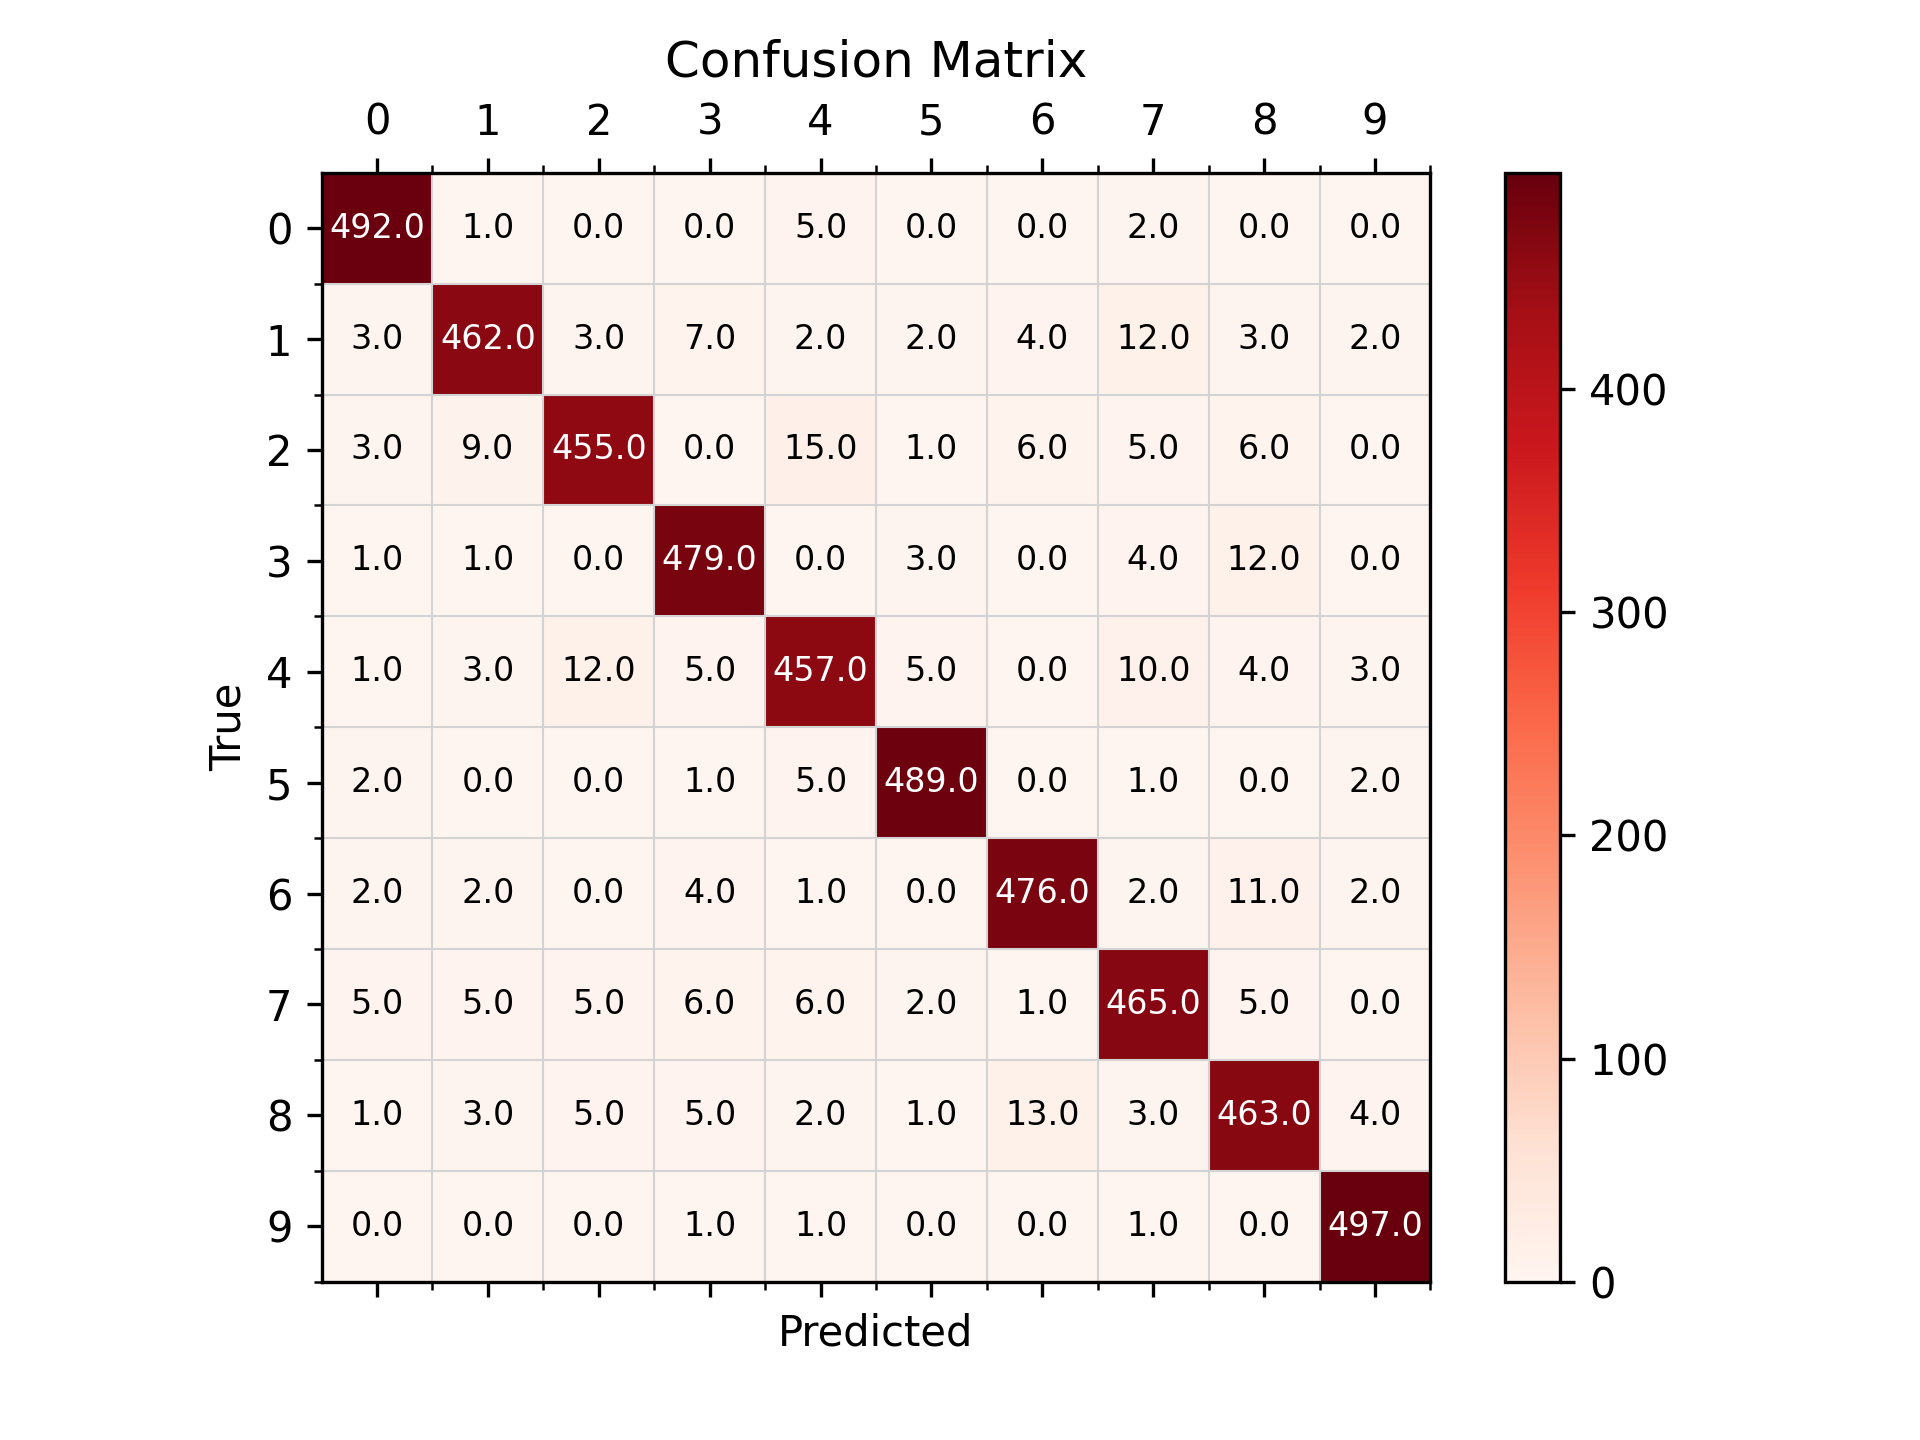
\includegraphics[width=0.7\textwidth]{./imagenes/confusion_matrix_one_vs_all.png}
    \caption{Matriz de confusión}
    \label{fig:matrix_a}
\end{figure}

\begin{figure}[H]
    \centering
    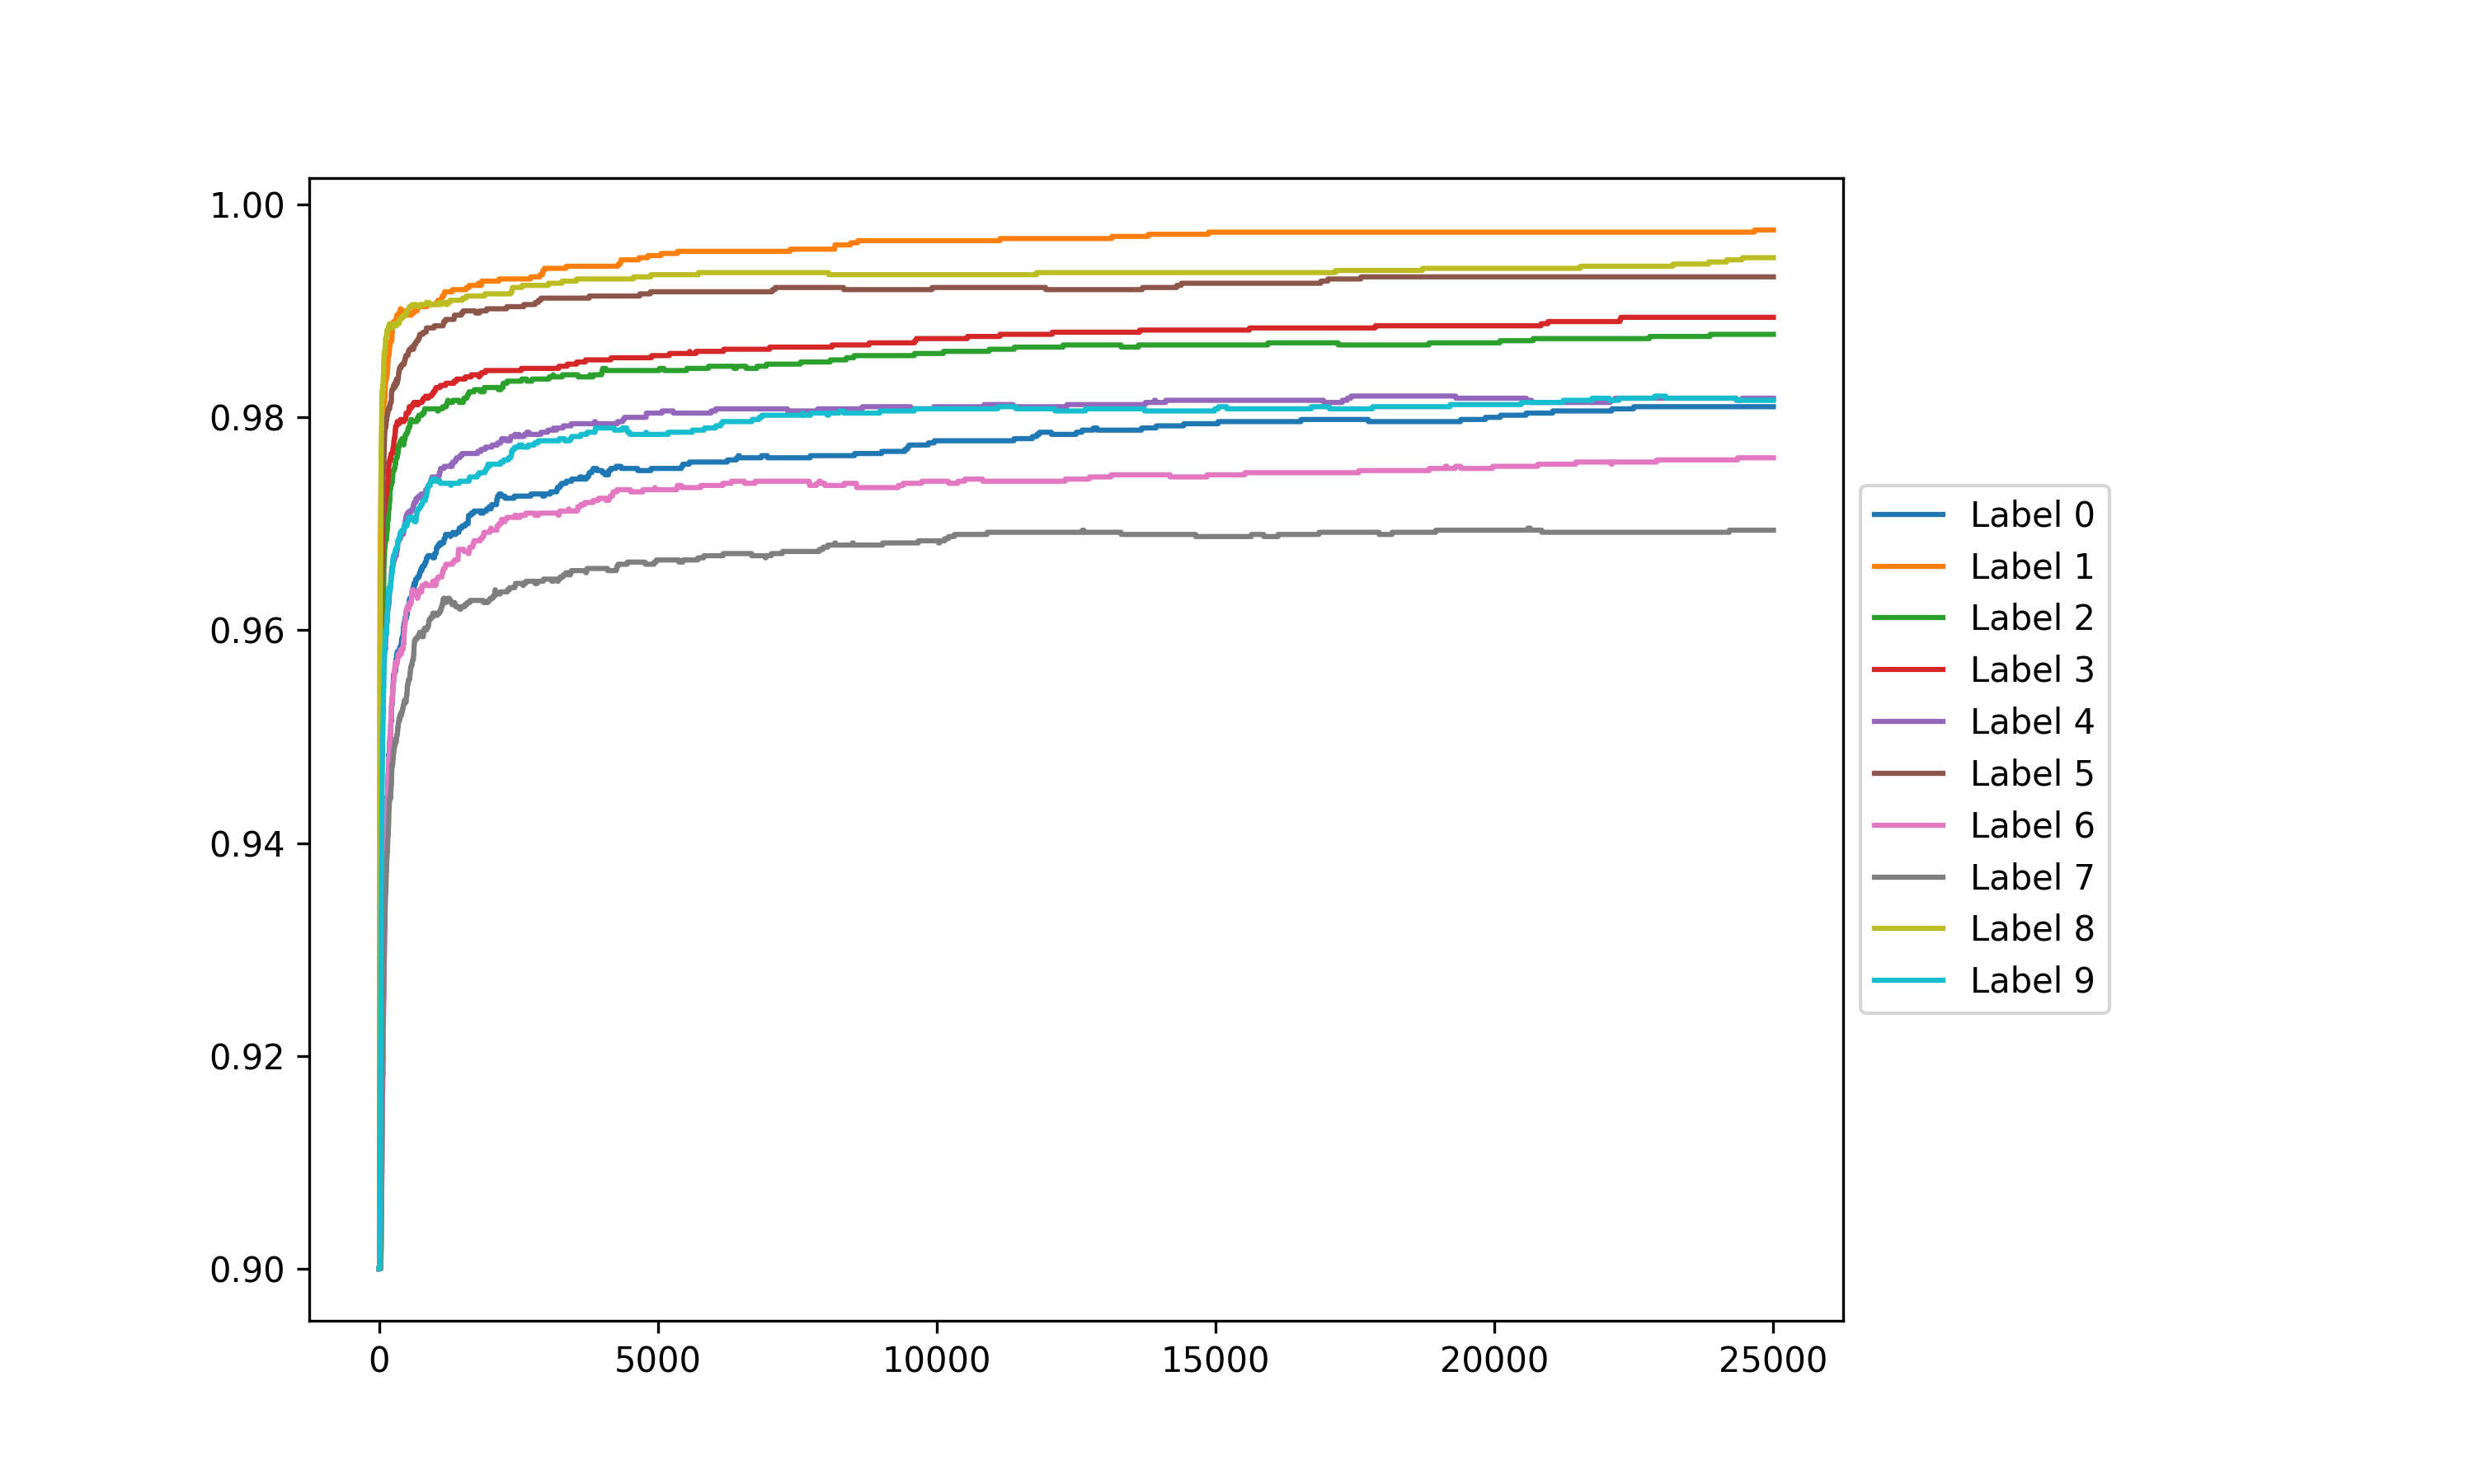
\includegraphics[width=0.7\textwidth]{./imagenes/predictions_one_vs_all.png}
    \caption{Predicciones}
    \label{fig:predictions_a}
\end{figure}

\begin{figure}[H]
    \centering
    \lstinputlisting[firstline=261,lastline=299, style=custompython]{../multi_class.py}
    \caption{Código de la función \textit{run\_one\_vs\_all}}
    \label{fig:run_one_vs_all}
\end{figure}

\begin{figure}[H]
    \centering
    \lstinputlisting[firstline=16,lastline=36, style=custompython]{../multi_class.py}
    \caption{Código de la función \textit{train\_model}}
    \label{fig:train_model}
\end{figure}

\begin{figure}[H]
    \centering
    \lstinputlisting[firstline=39,lastline=60, style=custompython]{../multi_class.py}
    \caption{Código de la función \textit{train\_all}}
    \label{fig:train_all}
\end{figure}

\begin{figure}[H]
    \centering
    \lstinputlisting[firstline=63,lastline=93, style=custompython]{../multi_class.py}
    \caption{Código de la función \textit{oneVsAll}}
    \label{fig:oneVsAll}
\end{figure}

\begin{figure}[H]
    \centering
    \lstinputlisting[firstline=96,lastline=128, style=custompython]{../multi_class.py}
    \caption{Código de la función \textit{predictOneVsAll}}
    \label{fig:predictOneVsAll}
\end{figure}

\begin{figure}[H]
    \centering
    \lstinputlisting[firstline=164,lastline=196, style=custompython]{../multi_class.py}
    \caption{Código de la función \textit{plot\_confusion\_matrix}}
    \label{fig:plot_confusion_matrix}
\end{figure}


\begin{figure}[H]
    \centering
    \lstinputlisting[firstline=219,lastline=241, style=custompython]{../multi_class.py}
    \caption{Código de la función \textit{print\_predictions}}
    \label{fig:print_predictions}
\end{figure}

\begin{figure}[H]
    \centering
    \lstinputlisting[firstline=199,lastline=206, style=custompython]{../multi_class.py}
    \caption{Código de la función \textit{save\_model}}
    \label{fig:save_model}
\end{figure}

\begin{figure}[H]
    \centering
    \lstinputlisting[firstline=209,lastline=216, style=custompython]{../multi_class.py}
    \caption{Código de la función \textit{save\_predict}}
    \label{fig:save_predict}
\end{figure}

\begin{figure}[H]
    \centering
    \lstinputlisting[firstline=244,lastline=258, style=custompython]{../multi_class.py}
    \caption{Código de la función \textit{save\_last\_predictions}}
    \label{fig:save_last_prediction}
\end{figure}

\section{Parte B: Regresión lógica regularizada}

En el apartado B usaremos el \textit{dataset} anterior, pero esta vez nos dan un modelo ya entrenado para hacer la red neuronal. Para ello usaremos la función \textit{predict} (figura \ref{fig:predict}) para hacer la predicción basándonos en el modelo dado. Usaremos la función de matriz de antes (\ref{fig:plot_confusion_matrix}) para hacer la matriz de confusión (figura \ref{fig:matrix_b}) y la función \textit{run\_neural\_network} (figura \ref{fig:run_neural_network}) para como driver de este apartado.

Tras ejecutar la red, conseguimos una predicción de 97.52\%.

\begin{figure}[H]
    \centering
    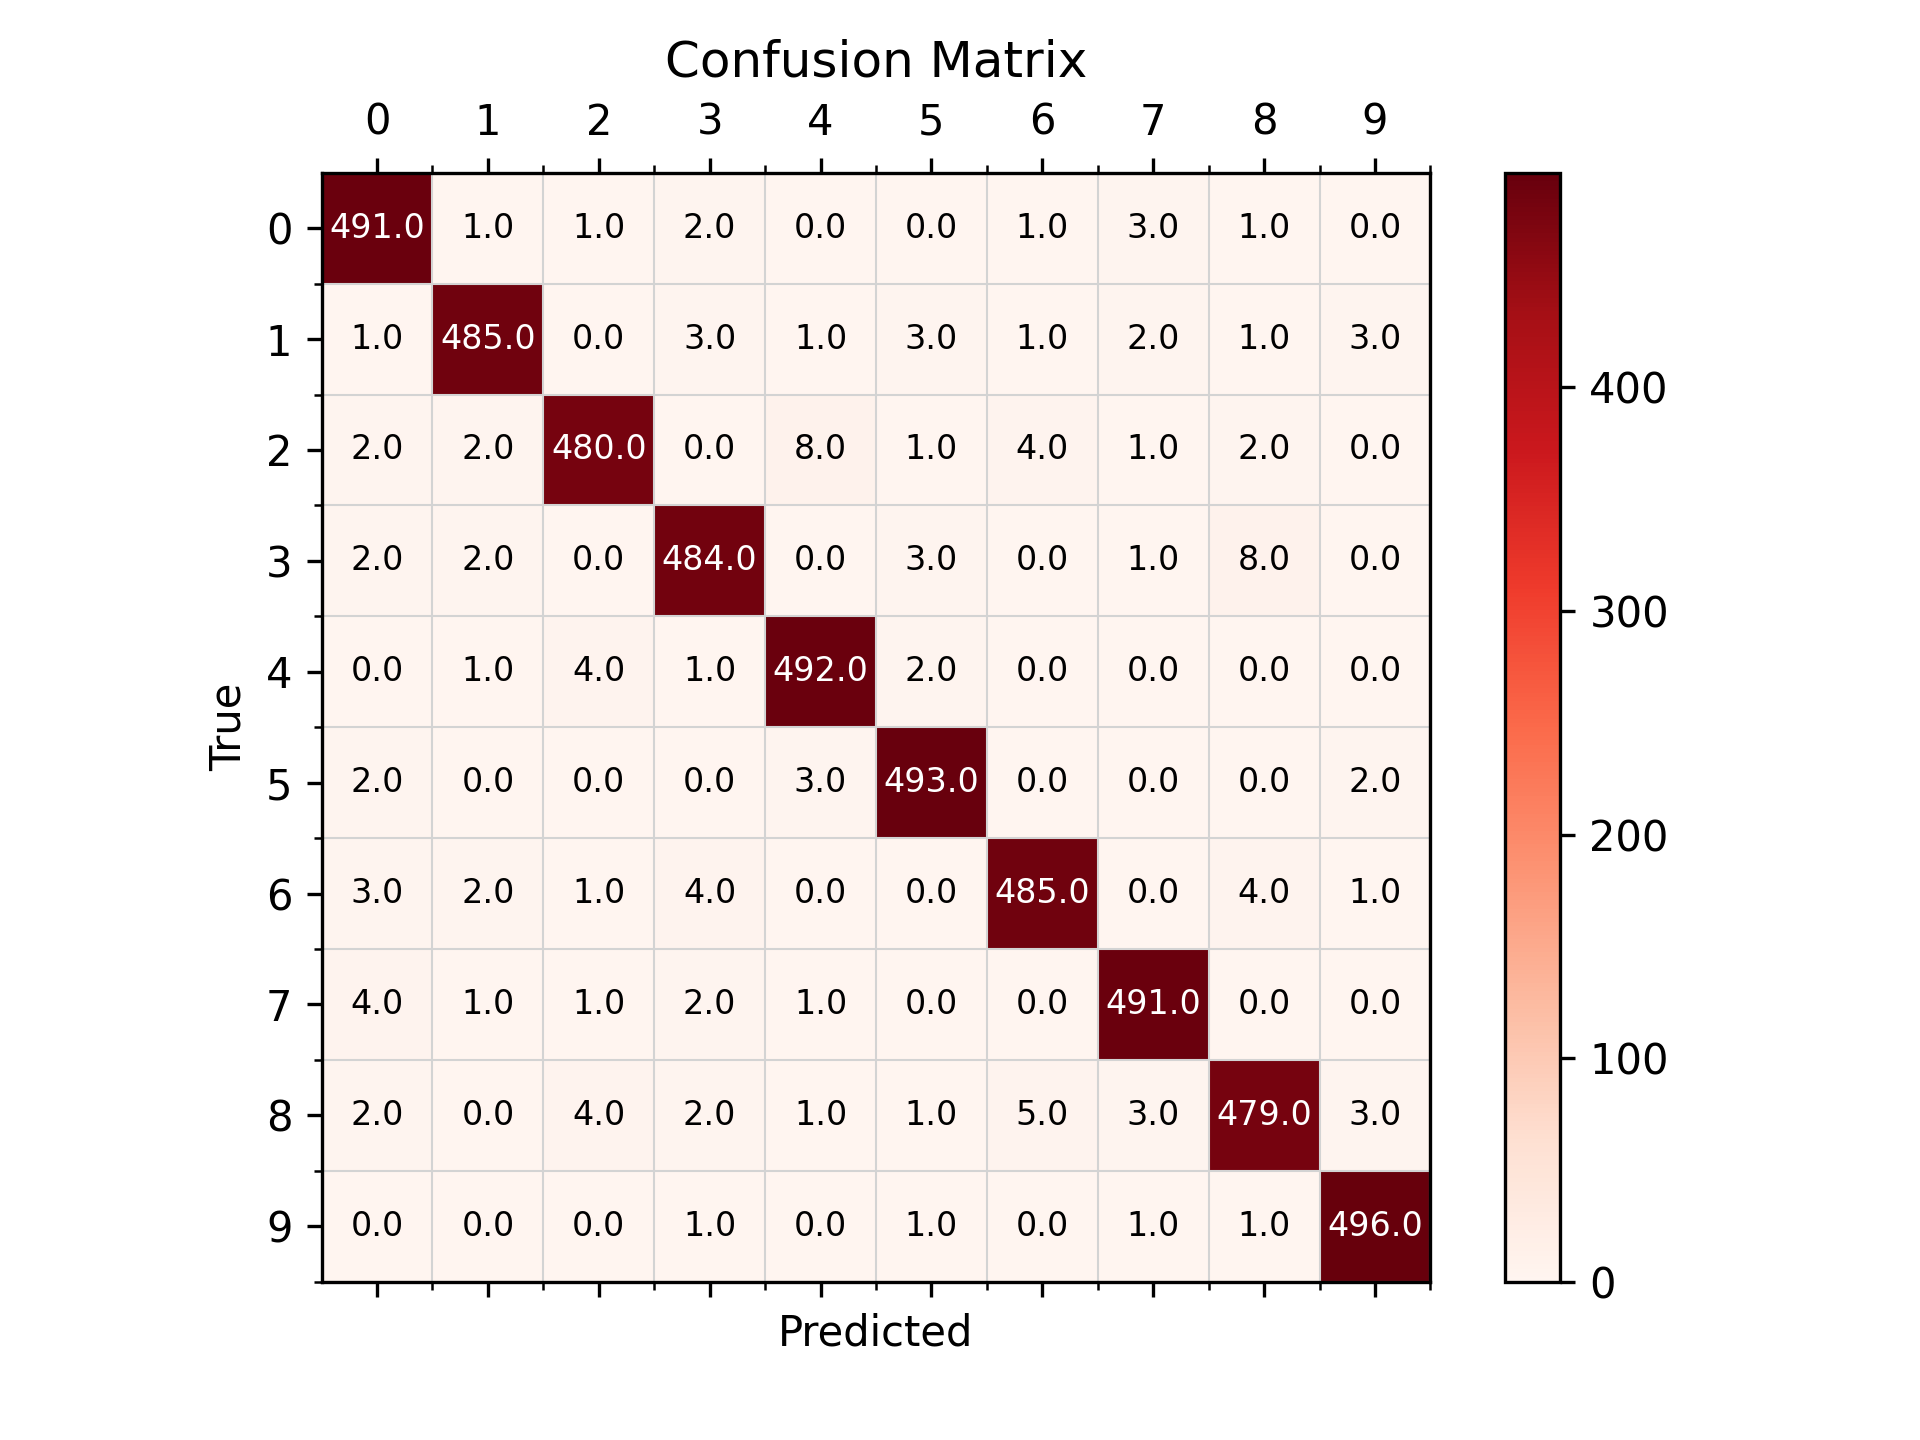
\includegraphics[width=0.7\textwidth]{./imagenes/confusion_matrix_nn.png}
    \caption{Matriz de confusión}
    \label{fig:matrix_b}
\end{figure}

\begin{figure}[H]
    \centering
    \lstinputlisting[firstline=134,lastline=161, style=custompython]{../multi_class.py}
    \caption{Código de la función \textit{predict}}
    \label{fig:predict}
\end{figure}

\begin{figure}[H]
    \centering
    \lstinputlisting[firstline=302,lastline=326, style=custompython]{../multi_class.py}
    \caption{Código de la función \textit{run\_neural\_network}}
    \label{fig:run_neural_network}
\end{figure}


\end{document}
